% What added knowledge do genomes contribute beyond case data w/o metadata?
% Transmission chains - spatio-temporal patterns of spread (already done, we just summarize here)
% Transmission chains - degree of super-spreading (we don't currently address this)
% Transmission chains - efficacy of contact tracing (observational and modelling studies give a range of values for efficacy, depending on implementation success. We get at CH implementation success, possibly compared to other countries, here.)

\documentclass[9pt,twoside,lineno]{pnas-new} % was: twocolumn

\makeatletter
\newcommand*{\addFileDependency}[1]{% argument=file name and extension
  \typeout{(#1)}
  \@addtofilelist{#1}
  \IfFileExists{#1}{}{\typeout{No file #1.}}
}

\usepackage{xr}
\addFileDependency{manuscript/text_supporting.tex}%
\addFileDependency{manuscript/text_supporting.aux}%
\externaldocument{manuscript/text_supporting}%

\usepackage{setspace}

\newcommand\focalcountry{CHE}
\newcommand\mindate{01. Jan. 2020}
\newcommand\maxdate{01. Dec. 2020}
\newcommand\maxmissing{2903}
\newcommand\minlength{27000}
\newcommand\maxsamplingfraction{0.05}
\newcommand\subsamplebycanton{TRUE}
\newcommand\travelcontextscalefactor{0}
\newcommand\similaritycontextscalefactor{2}
\newcommand\traveldataweights{1,1,1}
\newcommand\whichtrees{\.*}
\newcommand\pickchainsunderothercriteria{TRUE}
\newcommand\ntrees{-1}
\newcommand\smoothconfcases{FALSE}
\newcommand\outgroupgisaidepiisls{EPI\_ISL\_406798}
\newcommand\uniquecontextonly{FALSE}
\newcommand\maskfromstart{100}
\newcommand\maskfromend{50}

\newcommand\nchainsmin{746}
\newcommand\nchainsmax{2995}
\newcommand\minlargestchainsper{23}
\newcommand\maxlargestchainsper{14}
\newcommand\nspanningchainsmin{}
\newcommand\nspanningchainsmax{}

\newcommand\nfocalsamples{5520}
\newcommand\nsimcontext{11009}
\newcommand\ntravelcontext{0}
\newcommand\meanweeklysamplingpercent{NaN}
\newcommand\minweeklysamplingpercent{NaN}
\newcommand\maxweeklysamplingpercent{NaN}
\newcommand\overallsamplingpercent{1.4}

\newcommand\summer_max_dampling_percent_median_CHE_no_sampUB{37}
\newcommand\summer_min_dampling_percent_median_CHE_no_sampUB{65}


\templatetype{pnasresearcharticle} % Choose template 

\title{Genomic evidence for changes in Swiss SARS-CoV-2 transmission dynamics from public health measures and summer travel}

% Use letters for affiliations, numbers to show equal authorship (if applicable) and to indicate the corresponding author
\author[a,b]{Sarah A. Nadeau}
\author[a,b]{Timothy G. Vaughan} 
\author[b,c]{Emma B. Hodcroft} 
\author[b,d]{Richard A. Neher} 
\author[a,b,1]{Tanja Stadler}

\affil[a]{Department of Biosystems Science and Engineering, ETH Zürich, Basel, Switzerland}
\affil[b]{Swiss Institute of Bioinformatics, Lausanne, Switzerland}
\affil[c]{Institute for Social and Preventive Medicine, University of Bern, Bern, Switzerland}
\affil[d]{Biozentrum, University of Basel, Basel, Switzerland}

% Please include corresponding author, author contribution and author declaration information
% \authorcontributions{Please provide details of author contributions here.}
% \authordeclaration{Please declare any competing interests here.}
\correspondingauthor{\textsuperscript{1}To whom correspondence should be addressed. E-mail: tanja.stadler@bsse.ethz.ch}

% At least three keywords are required at submission. Please provide three to five keywords, separated by the pipe symbol.
\keywords{Epidemiology $|$ SARS-CoV-2 $|$ Phylogenetics $|$ Phylodynamics} 

\begin{abstract}
% Please provide an abstract of no more than 250 words in a single paragraph. Abstracts should explain to the general reader the major contributions of the article. References in the abstract must be cited in full within the abstract itself and cited in the text.
Pathogen genome sequences can help estimate transmission chains and, potentially, show how public health measures and travel effect transmission dynamics. Here we use SARS-CoV-2 sequences from approximately \overallsamplingpercent\% of all confirmed cases in Switzerland from the first case on 25. Feb. through \maxdate\ to quantify Swiss transmission dynamics through time. To do this, we used a two-step pyhylogenetic/phylodynamic framework and we report estimates across two extreme resolutions of phylogenetic uncertainty, acknowledging that SARS-CoV-2 sampling exceeds viral diversity. We show that in Spring 2020 SARS-CoV-2 was introduced many times prior to border closures, but subsequent measures drove most introductions to extinction. During Summer 2020, introductions rose as borders re-opened and this time many introductions persisted, driving high case numbers in Fall 2020. Finally, we show that in Summer 2020, Swiss transmission chains spread 40-60\% faster before first sampling than afterwards. We hypothesize this summertime ``burst-and-bust'' dynamic could be due to test-trace-isolate measures or denser contact networks surrounding returning travellers. Our analysis aims to help understand the importance of international travel towards a national epidemic, an increasingly relevant topic as global vaccination campaigns continue at an uneven pace and new variants of concern spread internationally.
\end{abstract}

\begin{document}

\maketitle
\abscontentformatted
\doublespacing

% \subsection*{Author Affiliations}

% Include department, institution, and complete address, with the ZIP/postal code, for each author. Use lower case letters to match authors with institutions, as shown in the example. PNAS strongly encourages authors to supply an \href{https://orcid.org/}{ORCID identifier} for each author. Individual authors must link their ORCID account to their PNAS account at \href{http://www.pnascentral.org/}{www.pnascentral.org}. For proper authentication, authors must provide their ORCID at submission and are not permitted to add ORCIDs on proofs.

\section{Introduction}

% Claim importance
A crucial task in public health is to evaluate measures aimed at slowing SARS-CoV-2 transmission. Such measures aim to prevent new introductions into a region or contain ongoing transmission chains, for example with quarantine for travellers or social distancing. So far, mathematical models have helped estimate effects from broad measures like travel bans and lockdowns. These methods use data on case or death counts and travel volumes, e.g. \cite{Flaxman2020, Tian2020}. However, these data aren't informative at the scale of individual introductions or transmission chains because there is no information to link related cases.

Detailed contact tracing data could help link cases to reconstruct introductions and transmission chains. However, these data are difficult to collect and sensitive. Instead, pathogen genome sequences can help link cases \cite{Kraemer}. Fast-mutating RNA viruses accumulate mutations on the same time-scale as host-to-host transmission. For example a typical SARS-CoV-2 strain will accumulate $\sim$2 mutations per month along its $\sim$30,000 nucleotide-long genome \cite{Nextstrainteam}. These mutations allow us to construct a viral phylogeny (a ``family tree'' of viruses) that approximates the underlying host-to-host transmission tree. 

SARS-CoV-2 genomes were collected at an unprecedented scale in 2020 \cite{Alm2020} and they have been used extensively to characterize transmission dynamics. Two broad categories of methods are commonly used: phylogenetic and phylodynamic methods. Phylogenetic studies reconstruct a ``best-guess'' phylogeny and calculate statistics directly from this phylogeny. For example, \cite{Mallon2020, DuPlessis2021} showed that national lock-downs during the early Irish and English epidemics reduced lineage sizes and diversity according to reconstructed phylogenies. On the other hand, phylodynamic studies assume the phylogeny must arise from some underlying model of transmission between hosts (and possibly migration between regions). This approach enables estimation of transmission dynamics. For example, \cite{Miller2020, Geoghegan2020a, Muller2020a} showed that public health measures reduced transmission rates in Israel, New Zealand, and Washington State, USA. Finally, \cite{Ragonnet-Cronin2021} took a different approach by comparing data across many regions. They showed a correlation between death counts and the delay between (phylogenetically-estimated) epidemic start and implementation of strong measures. Expanding on this wealth of prior work, we hope to quantify dynamics that are more directly relevant to public health measures.

% Indicate a gap
Unfortunately, it is quite tricky to make statements about public health measures using genomic data. Firstly, sequencing efforts vary by region and through time. Often, available samples are unrepresentative of the whole population \cite{Villabona-Arenas2020, DeMaio2015}. Secondly, SARS-CoV-2 sequencing was high compared to viral diversity, in particular during the early epidemic in Spring 2020. If many sequences are similar or identical the phylogeny contains unresolved polytomies. This means the phylogeny is only a coarse approximation of the  host-to-host transmission tree \cite{Villabona-Arenas2020}. Even worse, arbitrarily resolving polytomies may give misleading or overly confident estimates \cite{Morel2021}. Finally, real-world transmission dynamics are governed by complex population structure that is difficult to model. Highly parameterized phylodynamic models can help, as in \cite{Miller2020, Geoghegan2020a, Muller2020a}. Models with multiple compartments account for sampling biases and population structure and the phylogeny can be integrated out as a nuisance parameter. Recent developments are speeding these methods up \cite{Lemey2021}, but they are generally too computationally complex to fit to thousands of genomes.
% In the absence of strong prior information, these models are also too richly parameterized to be identifiable \cite{Louca2021FundamentalEpidemiology}.

% State that our paper fills the gap 
Here we present a two-step analysis framework carefully combing phylogenetic and phylodynamic methods to address these challenges. In each step, we condition on monophyletic partitions of the sample set, an approach inspired by  \cite{Muller2020} and \cite{DuPlessis}. This ensures computational feasibility. To limit sampling biases, we utilize sequences collected as part of the nation-wide Swiss SARS-CoV-2 genomic surveillance program. Namely, we sub-sample  available sequences to be more spatio-temporally representative of the Swiss epidemic. Finally, we conservatively report estimates across a range of plausible polytomy resolutions.

% Emphasize our main results 
We use our framework to quantify transmission dynamics in Switzerland, with a particular focus on the effects of travel and test-trace-isolate measures. First, we asked when introductions occurred and how long they persisted in Switzerland. We show that SARS-CoV-2 introductions were high prior to Spring 2020 border closures and increased again after these measures were relaxed in Summer 2020. Unlike in Spring, when new introductions were quickly driven to extinction during lockdown, these summertime introductions persisted over long periods and into Fall 2020. We then asked how well introductions were controlled once they were identified by public health authorities. We compared transmission rates pre- and post-first sampling as a proxy measure for the effect of test-trace-isolate campaigns. In Summer 2020 we estimate that transmission slowed 40-60\% after first sampling. We hypothesize this is due to test-trace-isolate measures and/or denser contact networks surrounding returning travellers. While we focus on epidemiological insights from the Swiss epidemic, our framework can be applied to any regional SARS-CoV-2 epidemic with data available on GISAID \cite{GISAID}. We perform a small comparison using New Zealand data to illustrate this. 

\section{Results}
We analyzed \nfocalsamples\ SARS-CoV-2 genomes collected in Switzerland, representing the Swiss epidemic from the first detected case on 25. Feb. through \maxdate. These data are a sub-sample of all available Swiss genomes aimed to be more spatio-temporally representative of the Swiss epidemic while maintaining a large sample size (Figure  \ref{fig:downsampling_representativeness}). 

\subsection{Introductions, then persistence drive the 2020 Swiss epidemic}

First, we constructed an approximate maximum-likelihood phylogeny for each SARS-CoV-2 Pango lineage, including Swiss sequences and the most genetically similar foreign sequences available on GISAID (Table \ref{tab:lineage-data-summary}). Within these lineage phylogenies, we identified introductions (both singleton samples and apparent transmission chains) as described in the Methods section. Importantly, we identify introductions under two extreme resolutions of phylogenetic uncertainty. This allows us to report estimates across the range of strictly bifurcating phylogenies consistent with the genome data. We refer to these extremes as ``few'' or ``many'' introductions.

We estimate the analyzed samples came from between \nchainsmin\ (few) and \nchainsmax\ (many) independent introductions into Switzerland. These introductions are roughly power law-distributed in size, with the 10 largest introductions accounting for \maxlargestchainsper\ to \minlargestchainsper \% of genome samples (Figure \ref{fig:chain_size_dist}). From a down-sampling analysis, we see that we do not reach saturation - if we were to include more genomes, we would identify more introductions (Figure \ref{fig:sensitivity_downsampling}). 

% For comparison: UK transmission lineages have power-law decay w/ alpha = 0.79 for chains 2 <= x <= 50, 1.26 for chains > 50. 
% Similar to Louis, I see chain sizes as power-law distributed, with a change in scale factor at ~ chain size 50. 
% The scaling factors I estimate are higher than his though (~1.2 for <= 50 and ~1.4 for >50). So, our Swiss chain sizes decay more sharply (fewer larger chains) than his UK transmission lineages.

Although the absolute number of introductions is very uncertain due to phylogenetic uncertainty and incomplete sampling, we expect trends through time to be more robust. Therefore, we focus on comparing new introductions and their persistence in Switzerland throughout 2020. Figure \ref{fig:chain-longevity} shows that the number of new introductions rose sharply from Feb. to Mar. 2020. This coincides with global SARS-CoV-2 infections rising in Feb. and Mar. 2020. Switzerland closed its borders from Mar. until Jun. 2020. New introductions dropped month-to-month during this time, from a high in Mar. to a low in Jun. 2020. Finally, new introductions rose more-or-less steadily from Jun. until Nov. 2020, coinciding with borders reopening across Europe and globally. 

New introductions cannot sustain an epidemic unless they persist in the local population. Genomic evidence suggests several introductions were quite persistent in Switzerland, including \nspanningchainsfebnovmin\ that may have persisted from the start of the Swiss epidemic in Feb. 2020 until Nov. 2020 (Figure \ref{fig:chain-longevity-matrix}). On average, the identified Swiss introductions persisted \meantimetolastsamplemax\ - \meantimetolastsamplemin\ days from first to last sampling. However, introductions in early 2020 were evidently less persistent than later introductions. Figure \ref{fig:chain-longevity} shows that $<$ 17\% of new introductions in Mar. and Apr. persisted more than 60 days while at least 9\% and up to 54\% of new introductions each month between Jul. and Sep. 2020 persisted this long.

% Finally, we can roughly estimate when introductions arrived as the date of the samples' most recent common ancestor (for transmission chains) or the sample date (for singletons). Introductions estimated to have arrived in the Swiss lockdown from 17. Mar. to 27. Apr. 2020 were more often singletons (63 - 85\% of introductions) than outside this period (31 - 72\%) \ref{tab:lockdown-contingency}.

\begin{figure}[H]
\centering
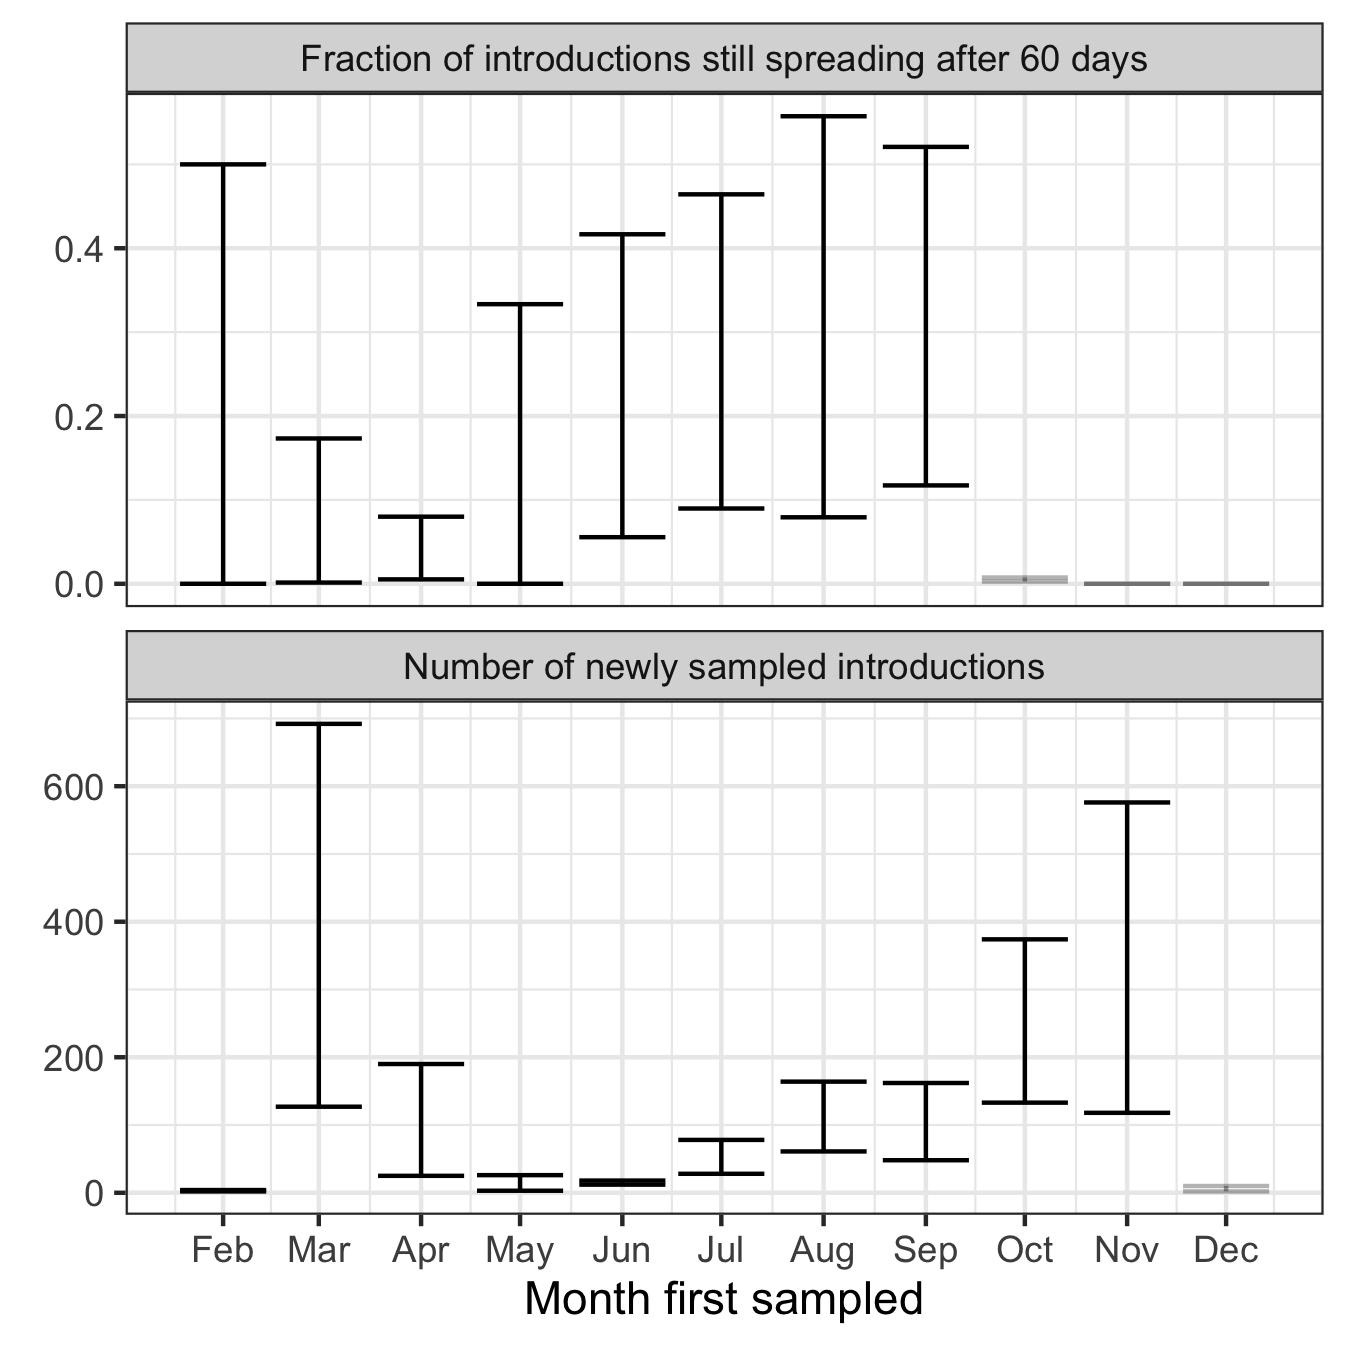
\includegraphics[width=.4\linewidth]{figures/introductions_and_persistance.png}
\caption{Introductions into Switzerland and their persistence by the month they were first sampled. Persistence is defined by $\geq$ 60 days between the first sample and the latest sample. The error bars span two point estimates generated assuming either few or many introductions.}
\label{fig:chain-longevity}
\end{figure}

\subsection{Genome data capture Summer 2020 ``breakpoint'' transmission dynamics}

Next, we inferred time-varying transmission dynamics within Switzerland in a Bayesian phylodynamic framework. The basic phylodynamic model is a birth-death with serial sampling model. In a nutshell, introductions are introduced into Switzerland some time before the first sample. All lineages transmit according to a time-varying effective reproductive number and are sampled with a time-varying sampling probability. The effective reproductive number is itself a function of a transmission rate parameter and a becoming-uninfectious rate parameter. We fixed the becoming-uninfectious rate to improve model identifiability. Therefore, the effective reproductive number varies only with the transmission rate. We fit this model to infer transmission parameters jointly from either the ``few'' or ``many'' identified introductions.

On top of this model, we added a transmission rate ``damping'' factor. This aims to test whether test-trace-isolate efforts in Switzerland slowed transmission once an introduction was detected. Given there is no travel-related quarantining or altered testing, we reasoned test-trace-isolate could slow transmission shortly after the first case tests positive but not beforehand. We include this concept in our model by allowing the transmission rate to decrease at 2 days after each introduction is first sampled by a multiplicative factor. We used a spike-and-slab prior on this factor to include the possibility of no transmission slow-down. To test robustness, we repeated the analysis under several different model configurations (Table \ref{tab:phylo-models}).

Across all models and assuming either ``few'' or ``many'' introductions, we get effective reproductive number estimates that roughly capture the same trends as estimates based on confirmed case counts (Figure \ref{fig:ReSampProbResults}). On the other hand, sampling probability estimates in Fall 2020 are strongly dependent on the prior (Figure \ref{fig:ReSampProbResults}).

SARS-CoV-2 genome data additionally provide a unique view on introduction-specific transmission dynamics. We estimate a \summermaxdamplingpercentmedianCHEnosampUB\ - \summermindamplingpercentmedianCHEnosampUB\% slow-down in transmission after introductions are first sampled during Summer 2020. In comparison, we estimate no or very little slow-down in relation to first sampling during Fall 2020 (Figure \ref{fig:scale-factor}). These results are qualitatively robust to assuming few or many introductions, imposing a strong prior bound on the sampling proportion, and including a second deme of super-spreading individuals in the model (Figure \ref{fig:DampingFactorResults}). In contrast, estimates in Spring 2020 are inconsistent. This could be explained by low genomic diversity in SARS-CoV-2 contributing to high phylogenetic uncertainty; figures \ref{fig:logged-chains-min}, \ref{fig:logged-chains-max} give examples of how transmission dynamics within Spring 2020 introductions vary greatly depending on introduction definition. In summary, we report an evident ``breakpoint'' dynamic in SARS-CoV-2 transmission in Switzerland in Summer 2020 where transmission evidently slows shortly after the first sample is generated.

\subsection{Comparison to the New Zealand epidemic}
While Switzerland is centrally located in Europe and well-connected to other countries, especially those in the (normally) barrier-free Schengen travel zone, New Zealand is a relatively isolated island nation. Additionally, New Zealand aimed to eradicate SARS-CoV-2 throughout 2020 using strong measures, such as keeping it's borders closed, while Switzerland re-opened to Europe in early Summer 2020. We compared our estimates for the transmission slow-down factor between Switzerland in Spring, Summer, and Fall 2020 with New Zealand before and after local transmission was all but eradicated there in mid-May 2020. Estimated damping factors in New Zealand before and after 15. May were comparable or stronger than in Switzerland during Summer and Fall 2020 (Figure \ref{fig:scale-factor}).

\begin{figure}[]
\centering
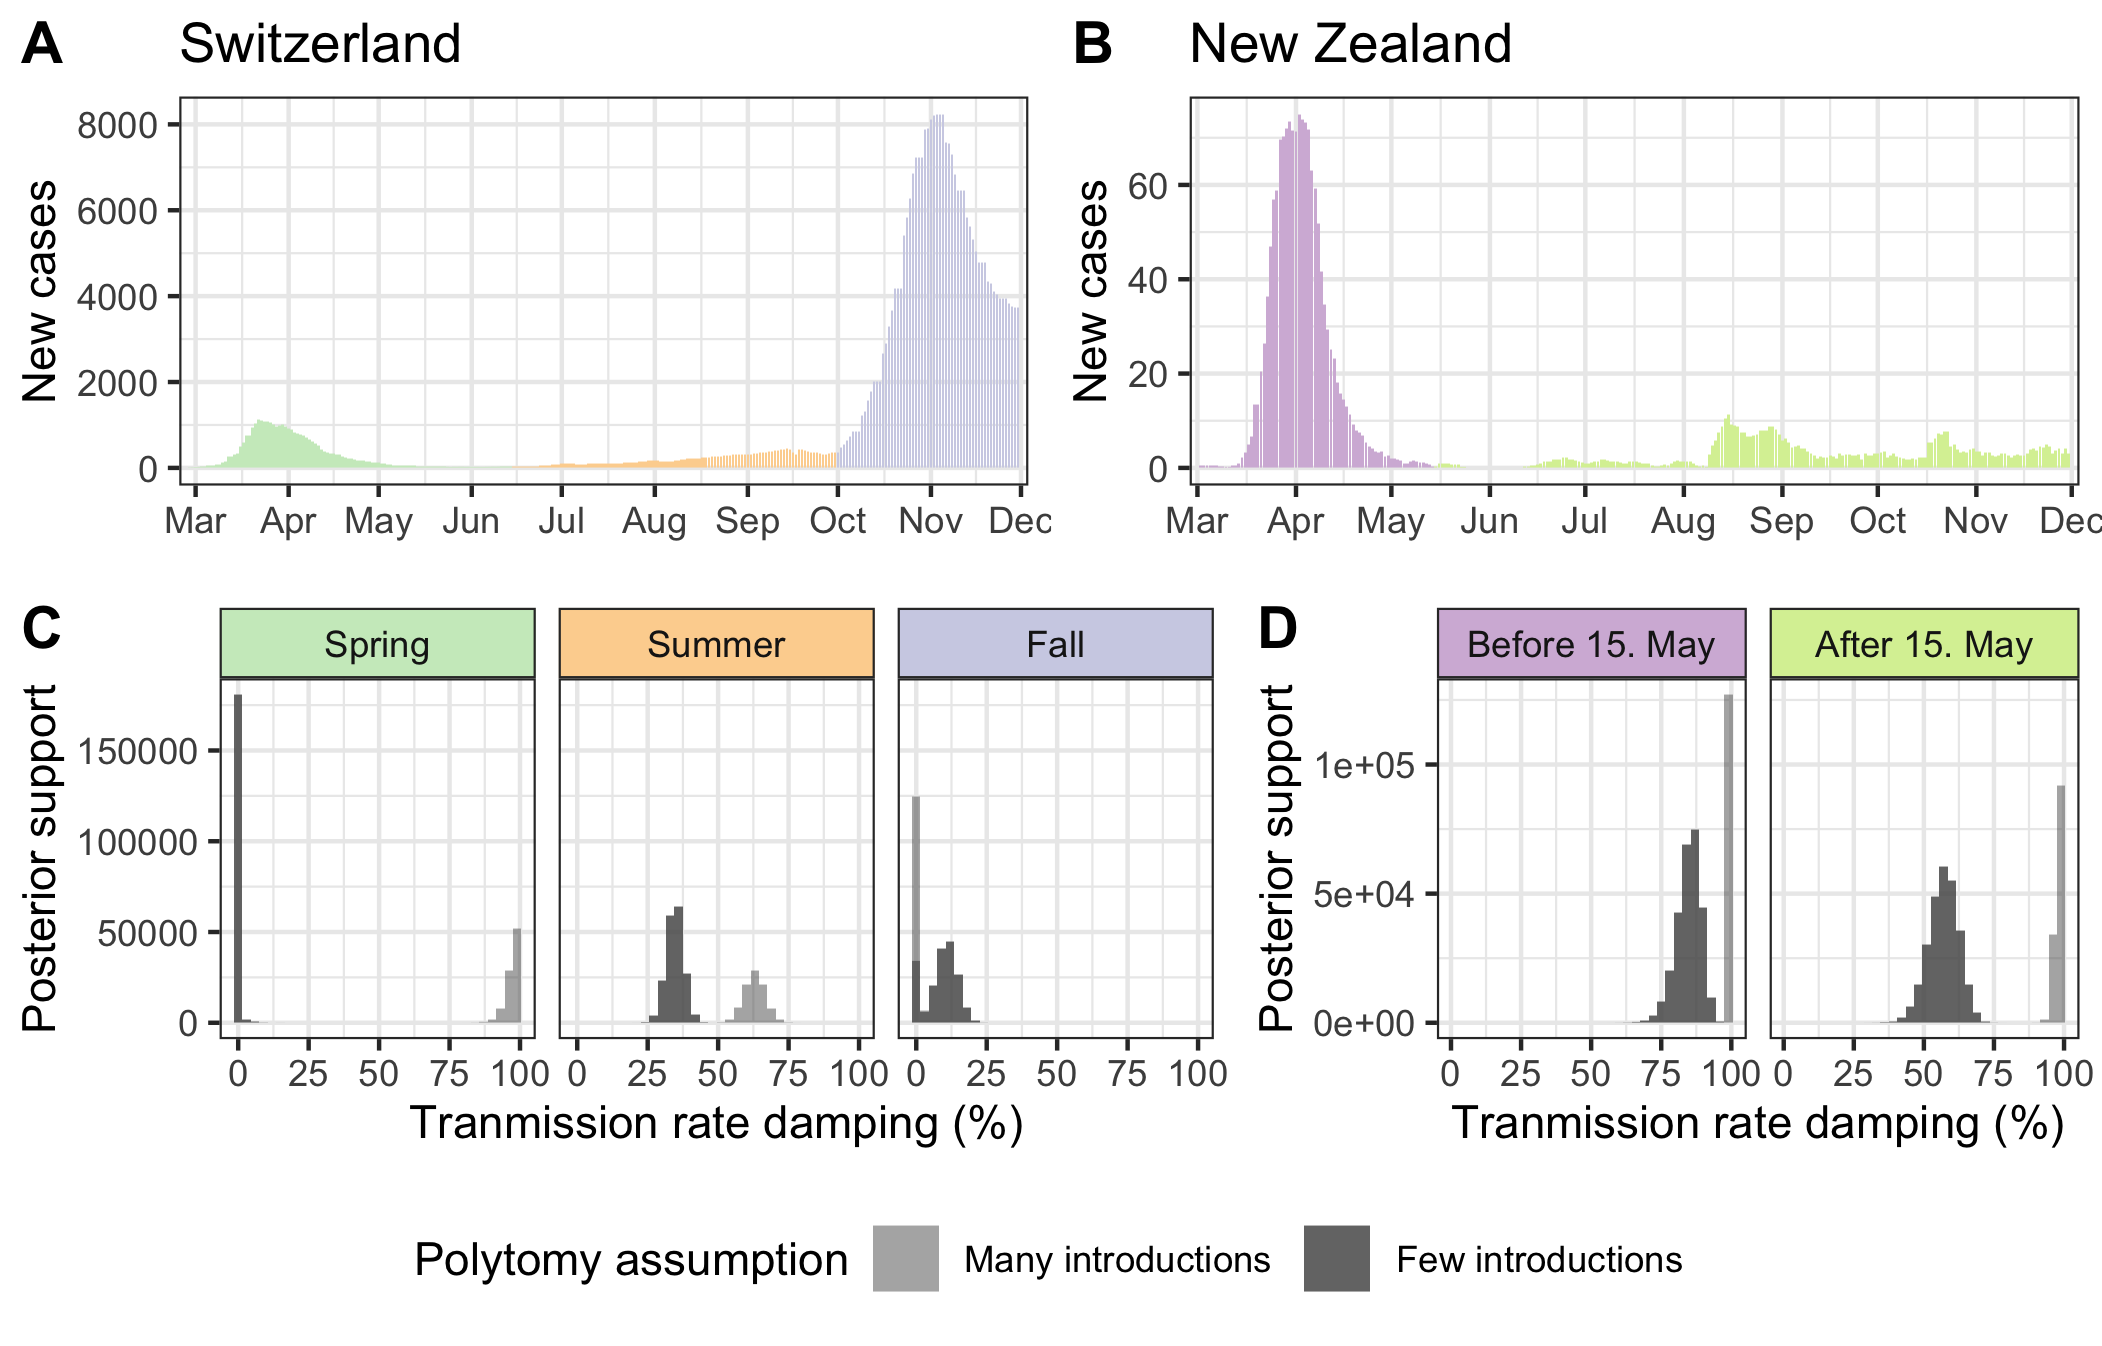
\includegraphics[width=\linewidth]{figures/contact_tracing_factors_no_sampUB_compared_to_cases.png}
\caption{Estimated reduction in the effective reproductive number Re once introductions have been sampled (top) during three different time periods characterised by different case loads in Switzerland (bottom). Estimates were generated twice, once conditioning on few introductions and once conditioning on many introductions.}  
\label{fig:scale-factor}
\end{figure}

\section{Discussion}
% Re-state the goal and the main results
We aimed to assess genomic evidence for the impact of public health measures on SARS-CoV-2 transmission in Switzerland. The most conservative interpretation of our results indicates that after Swiss borders were partially closed from 25. Mar. 2020, the number of newly sampled lineages per month dropped 83\% from Mar. to Jun. 2020. These measures were mostly lifted again on 14. Jun 2020. Correspondingly, we estimate at least a 31\% increase in newly sampled lineages from Jun. to Jul. 2020. Further, during the Swiss lockdown from 17. Mar. to 27. Apr. 2020, introductions were 13 or 32\% more likely to be singletons than outside this period. Finally, we estimate that the reproductive number of introductions dropped 40 - 60\% after sampling during Summer 2020 in Switzerland, possibly due to test-trace-isolate success upon detection. We interrogate and contextualize this result below, as we cannot exclude other possible explanations for this estimated transmission slow-down.

% Argue for utility
First, we argue the two-step analysis framework we developed may be useful to others since it enables rapid analysis of national-size data sets. In particular, the phylogenetic analysis uses semi-public data from GISAID and requires limited computational resources. To reduce data set size and computation time, one can increase sub-sampling, reduce the time-frame of interest, or specify a subset of Pango lineages using a yaml-formatted configuration file. The implementation currently relies on an in-house database based on GISAID and other external data sources. Soon, we will adapt it to use a public API based on fully public data from GenBank hosted by Nextstrain (LAPIS). Users will set configurations via the single configuration file and then the analysis can be run via Docker or Singularity without further modification.

% Contextualize the results: caveats
Next, we'll address the limitations of the phylogenetic and phylodynamic methods we used. Most obviously, estimates on the number, timing, and duration of introductions are very uncertain due to polytomies in the phylogeny. Others have struggled with the same challenge \cite{Morel2021} and we support their conclusion: one should consider estimates generated across a range of plausible phylogenies, as estimates based on any one phylogeny may be misleading. In our analysis, we present estimate ranges based on two extreme resolutions of polytomies. This is less computationally intensive, but perhaps overly conservative, compared to generating a larger set of plausible phylogenies as in Bayesian analyses and as \cite{Morel2021} suggested for maximum-likelihood analyses.

Further, genomic data are observational data subject to potential sampling biases. The benefit of genome data is that we can aim to quantify the real-world effect of public health measures like test-trace-isolate. This distinguishes our work from simulation studies aiming to quantify a theoretical effect. However, genome data may not represent the overall infected population due to time-varying testing regimes, geographic sampling biases, and demographic skew in disease severity. In particular, we expect severe cases, contacts of positive cases, and large transmission chains are more likely to be sampled. If we assume these biases are constant through time, we can focus on interpreting trends in transmission dynamics through time. 

Finally, we cannot unequivocally attribute the estimated slow-down in transmission upon sampling to test-trace-isolate success. Returning travellers have been implicated in transmitting more than non-travellers \cite{Hodcroft2021}. A passive slow-down in transmission might happen as the virus moves into the non-traveller population. To this end, we repeated our analysis using data from New Zealand, where all travellers were quarantined since TODO. In New Zealand, we estimate comparable or stronger slow-downs in transmission before and after 15. May 2020 compared to Summer and Fall 2020 in Switzerland. Since New Zealand travellers could not mix normally with non-travellers, at least in New Zealand these slow-down effects should be from quarantine. We also noted that contacts of positive cases and members of large transmission chains are more likely to be sampled. This means we might sample bursts of transmission, possibly due to super-spreading, which are again followed by a passive slow-down in transmission once a super-spreading event is over or a super-spreader is no longer infectious. However, in this case we would expect periodic bursts of super-spreading-related samples to occur regardless of whether an introduction is recently sampled or not. We would also expect super-spreading to continue into Fall 2020, when case counts were high in Switzerland, but the slow-down factor is only significant in Summer 2020, when case counts were low. Therefore, we suspect test-trace-isolate and quarantine measures help mitigate onward transmission from introductions. Phrased more conservatively, we can quantify "burst-and-bust" SARS-CoV-2 transmission dynamics in Summer 2020 in Switzerland and in New Zealand.

% Argue for importance
Our findings are important because they highlight the effect of public health measures on the Swiss epidemic. We show that strict public health measures like the partial border closure and lockdown in Spring 2020 helped prevent and contain new introductions. However, these measures are naturally unsustainable. We show that when case counts are maintained at a low level, as in Summer 2020 in Switzerland and after 15. May in New Zealand, new introductions initially spread more quickly, but then slow down. Estimates from Fall 2020 in Switzerland indicate that no such slow-down occurs when case counts are high. We speculate this is due to test-trace-isolate resources being overwhelmed. In conclusion, our results argue for the benefits of continued test-trace-isolate effects, thoughtful quarantine policies, and aiming to maintain case counts at a low level.

\section{Acknowledgments}

\begin{itemize}
    \item Jana: discussions about how test-trace-isolate affects sampling
    \item Viollier: in particular Christiane for providing data and logistical support
\end{itemize}

\section{Methods}
\subsection*{Genome sequencing and quality filtering}
Most of the Swiss SARS-CoV-2 genomes analyzed until 31. Dec 2020 were generated by the Swiss SARS-CoV-2 Sequencing Consortium. Here, we briefly describe the swab-to-sequence process for these samples. RNA extracts from qPRC-positive patient naso- or oral-pharangeal swabs were provided by Viollier AG, a Swiss medical diagnostics company. RNA extraction was done with either the Abbott m2000sp or Seegene STARMag 96x4 Universal Cartridge RNA extraction kit. Extracts were then  transferred to the Genomics Facility Basel or the Functional Genomics Center Zurich for whole-genome sequencing. Both centers used the ARCTIC v3 primer scheme \cite{Quick2017, ARCTICNetwork} to generate tiled, approximately 400bp-long amplicons. Library preparation was done with the New England Biolabs (NEB) library preparation kit. Libraries were sequenced on Illumina MiSeq or NovaSeq machines, resulting in 2 x 251 base reads. Bioinformatics was done using V-pipe \cite{Posada-Cespedes2020}, including read trimming and filtering with PRINSEQ \cite{Schmieder2011}, alignment to Genbank accession MN908947 \cite{Wu2020} with bwa \cite{Li2009}, and consensus base calling. For consensus base calling, positions with $<$5x coverage are masked with ``N'', positions with $>$5\% and $>$2 reads supporting a minor base are called with IUPAC ambiguity codes, and positions with $>$50\% reads supporting a deletion are called with ``-''. We rejected samples with $<$20,000 non-N bases. The consensus sequences we generated have been made publicly available on both GISAID (submitting lab: Department of Biosystems Science and Engineering, ETH Zürich) and ENA (study: PRJEB38472).

We supplemented our Swiss data with other Swiss sequences and foreign sequences available via GISAID (accessed 31. May 2021). From the full set of sequences available on GISAID, we removed from consideration non-human samples, samples $<$ 27000 bases long, and samples flagged by the Nextclade tool \cite{Aksamentov} for one of the following reasons: suspiciously clustered SNPs (QC SNP clusters status metric not ``good''; $>=$ 6 mutations in 100 bases), too many private mutations (QC private mutations status metric not ``good''; $>=$ 10 mutations from the nearest tree node), or overall bad quality (Nextclade QC overall status ``bad''). We aligned the sequences to the reference genome MN908947.3 using MAFFT \cite{katoh_mafft:_2002}. Finally, we followed the Nextstrain pipeline's recommendation to mask the first 100 and last 50 sites of the alignment \cite{Nextstraina} since the start and end of SARS-CoV-2 sequences are prone to sequencing error \cite{DeMaio2020}.

\subsection*{Sampling procedure}

From the quality-filtered alignment of GISAID sequences, we selected a focal set of sequences from Switzerland and a context set of sequences from abroad. 

% describe representativeness of Swiss dataset here too?
For the focal sequences from Switzerland, we aimed to select a spatially and temporally representative sample. Therefore, we down-sampled available sequences to \maxweeklysamplingpercent\% of confirmed case counts in each Swiss Canton each week between \mindate\ and \maxdate. Where there were not enough sequences available from a Canton in a week, we took the maximum available sequences. To reduce the size of the alignments for phylogenetic analysis, we divided the focal Swiss set into Pango lineages \cite{Rambaut}, similar to \cite{DuPlessis2021}. Lineages composed of $>=$ 50\% Swiss sequences were aggregated into their parent lineage(s) until $<$ 50\% were Swiss. This aims to ensure that each analyzed lineage originated outside of Switzerland.

% describe nextstrain priority protocol for sim dataset
For the context sequences from abroad, we aimed to select the most genetically similar sequences to focal Swiss sequences. This set should help distinguish between SARS-CoV-2 strains unique to Switzerland (likely within-Switzerland transmission) and strains also circulating abroad (possibly recent introductions). To select this set, we applied the Nextstrain priority script \cite{Nextstrain} to rank sequences from abroad by their genetic similarity to Swiss sequences in each lineage alignment. Then, we selected \similaritycontextscalefactor times as many most context sequences as focal Swiss sequences for each analyzed lineage. 

% summarize the sample set
The final dataset for analysis includes \nfocalsamples\ focal sequences from Switzerland and \nsimcontext\ genetically similar context sequences from abroad.

\subsection*{Timetree generation}
We estimated the maximum likelihood phylogeny for each lineage alignment using IQ-TREE \cite{Nguyen2014} under an HKY substitution model \cite{Hasegawa1985} with empirical base frequencies and 4 gamma rate categories. We then rooted each phylogeny with \outgroupgisaidepiisls\ as an outgroup and estimated branch lengths in time units using least-squares dating (LSD) \cite{To2016} with a strict molecular clock and a minimum mutation rate of 8x10-4 substitutions per site per year. We additionally assumed the root date to be between 15. Nov. and 24. Dec. 2019 (roughly in line with estimates provided by Nextstrain \cite{Nextstrainteam}) and set the minimum branch length to zero. Sequences that violated the strict clock assumption (z-score threshold > 3) were removed and near-zero branches ($<$1.7x10-5 substitutions per site per year) were collapsed into polytomies, reflecting the fact that the sequence data is not sufficient to resolve the ordering of these transmission events. Given the root date constraints, the mutation rate conformed to the lower bound of 8x10-4 with extremely narrow confidence intervals. Confidence intervals for node dates were generated in LSD by re- sampling branch lengths 100 times under a lognormal relaxed clock model with standard deviation 0.4.

\subsection*{Phylogenetic analysis}
We ``picked'' putative Swiss transmission chains off of each Pango lineage tree according to the following criteria: at least 2 Swiss sequences are part of a clade in the tree and the subtree spanned by these Swiss sequences is monophyletic upon removing (a) up to 3 export events where (b) only one export event may occur along each internal branch. Exports are defined to be clades containing non-Swiss sequences. We chose a conservative value for criterion (b) while still allowing some export events and note that the number of inferred transmission chains is robust to different values for criterion (a) given criterion (b) (Fig. S13).

We repeated our analysis interpreting polytomies in two ways. Once, we split Swiss clades descending from polytomies unless the polytomy only had a single non-Swiss descendent (see criterion (b)). Alternatively, we aggregated all Swiss clades descending from polytomies into a single transmission chain. These procedures represent two plausible extremes, the first being maximum introductions and minimum local transmission and the second being minimum introductions and maximum local transmission.

We refer to any Swiss sequence not falling into a Swiss transmission chain as a Swiss singleton. We assume each singleton and each transmission chain represent an independent introduction of SARS-CoV-2 into Switzerland; together these are called introductions.

% Date of each introduction?

\subsection*{Phylodynamic analysis}

Here, we do not focus on estimating the effective reproductive number or the sampling proportion. Instead, we concentrate on insights that can only be generated by considering individual transmission chains. The effective reproductive number can be well-estimated using confirmed case data in Switzerland \cite{, huisman_re_preprint}. Further, we argue the sampling proportion should be treated as a fitting parameter, since testing strategies varied through time in Switzerland and information from serological studies in different regions and at different time-points are difficult to harmonize. However, we did test for robustness to a strong prior on the sampling probability based on confirmed case counts and results are qualitatively similar (Figure \ref{fig:ReSampProbResults}).

We performed inference under several different models, all implemented using the BDSKY package \cite{stadler2013birth} in BEAST2 \cite{Bouckaert2019}, which assumes a birth-death population dynamical model. In all the models, we conditioned on identified introductions, as in \cite{Muller2020}, and estimated parameters jointly from the different introductions. More concretely, each introduction is assumed to result from an independent birth-death process having its own start time, but sharing all other parameters with the processes associated with the other introductions. To avoid model mis-specification due to the more transmissible alpha variant, we analyzed data only through 30. Nov. 2020. We fixed the expected become-uninfectious rate to 36.5 per year, which corresponds to an average time to becoming uninfectious of 10 days. We assumed an HKY \cite{Hasegawa1985} nucleotide substitution model with 4 gamma rate categories to account for site-to-site rate heterogeneity \cite{Yang1994}. We assumed a strict clock, also with rate 8x10-4 substitutions per site per year. We applied a uniform prior from 01. Jan to 31. Dec 2020 to the time of origin for each introduction, so that our prior expectation is a uniform rate of introductions through time. The effective reproductive number was allowed to vary according to an Ornstein-Uhlenbeck prior with a LogNormal(0.8, 0.5) stationary distribution. An Exp(1) hyperprior was applied to the variance of the Gaussian component of the smoothing prior. This prior constrains both the relative sizes of the change between weeks and the absolute reproductive number. The sampling proportion was allowed to vary at time points when Swiss testing or genome sampling regimes changed significantly (Table \ref{tab:CHE_samp_prob_change_dates}). Depending on the analysis, we specified either a LogUniform(0, 1) or LogUniform(0, 0.05) prior on the sampling proportion, since we upper-bounded our sampling to 5\% of confirmed cases each week.

Our ``contact tracing'' model included one additional parameter, a multiplicative down-scaling of the effective reproductive number applied to each introduction from 2 days after the first sample date until the last sample in the introduction. Since we suspected contact tracing was not functioning as well during periods of high case numbers, we estimated a separate value in each of three periods: before 15. Jun 2020, 15. Jun to 30. Sept 2020, and 30. Sept to \maxdate. The same spike and slab prior was applied to the contact tracing factor in each period, with a prior inclusion probability of ?? and a uniform prior if included between 0 and 1. The XML file including these modification is available at TODO.

Our ``super-spreading'' model included an additional deme, representing a fraction of the population that transmits faster. A multiplicative up-scaling of the effective reproductive number is applied to individuals in this deme.

\acknow{This work was supported by the Swiss National Science Foundation (SNSF) through grant number 31CA30\_196267 (to TS).}

\showacknow{} % Display the acknowledgments section

% Bibliography
\bibliography{references}

\end{document}
